\documentclass[dvipsnames,unknownkeysallowed,10pt,brazil]{beamer}
%
%
%  Para configurar, procure por ``muda''
%
%
\usepackage{babel}
\usepackage{calc}
\usepackage{ifthen}
\usepackage[T1]{fontenc}
\usepackage{xcolor}
\usepackage{tikz}
\usepackage{tikz-3dplot}
\usepackage{pgfplots}
\usetikzlibrary{3d,arrows,babel,calc,angles,quotes,patterns}
\usepackage{pgf}
\usepackage{pgffor}
\usepackage{cancel}
\usepackage{amsmath}
\usepackage{wasysym}
%\usepackage{marvosym}
\usepackage{tikzsymbols}
\usepackage{graphicx}
%\usepackage{algorithm2e}
\usepackage{algpseudocode}
\usepackage{nicefrac}
\usepackage{siunitx}
\usepackage{multirow}
\usepackage{multicol}
\usepackage{colortbl}
\usepackage{enumerate}
\usepackage{multimedia}
\usepackage{listings} 
\usepackage{hyperref}
\usepackage{verbatim}
\usepackage{zi4}
\usepackage{fontawesome}
\usepackage{fancyvrb}
\usepackage[utf8]{inputenc}
\usepackage{systeme,mathtools}
%\usepackage[eulergreek,italic,defaultmathsizes]{mathastext}


\graphicspath{{./} {./figures/}}
% set text colors for different objects
\colorlet{grey}{white!65!black}
% \colorlet{base}{orange!80!black}
\colorlet{mat}{Plum}
%
% muda
%
\definecolor{amber}{rgb}{1.0, 0.75, 0.0}
\definecolor{base}{RGB}{78,15,92}
\definecolor{fundo}{RGB}{133,52,150}
\definecolor{giz}{rgb}{0.85,0.85,0.85}

\setbeamercolor{frametitle}{bg=base,fg=white}
\setbeamercolor{framesubtitle}{fg=black}
\setbeamercolor{structure}{fg=black}
\setbeamercolor{normal text}{fg=black}
\setbeamercolor{alerted text}{fg=red}
\setbeamercolor{example text}{fg=black}
\setbeamercolor{math text}{fg=base}
\setbeamercolor{math text displayed}{fg=mat}
\setbeamercolor{math text inlined}{fg=mat}
\setbeamercolor{item projected}{bg=base}
\setbeamertemplate{enumerate items}[default]
\setbeamercolor{local structure}{fg=base}
\everymath{\color{base}}

%% set fonts
%\usefonttheme{professionalfonts}
\usepackage[sfdefault,lf]{FiraSans}
\setbeamerfont{frametitle}{size=\Large,series=\firasemibold,shape=\scshape}
\setbeamerfont{framesubtitle}{shape=\scshape}
\setbeamerfont{title}{size=\Huge,series=\firasemibold}
\setbeamerfont{author}{size=\Large,series=\bfseries}
\setbeamerfont{date}{size=\large}
\setbeamerfont{institute}{size=\large,series=\firasemibold}
\newcommand\ttblue[1]{\textcolor{Plum}{\texttt{#1}}}
%\usepackage[sfdefault,lf]{carlito} %% option 'sfdefault' activates Clear Sans as the default text font
%\usepackage{newtxsfs}
\usepackage{mathpazo}
%\usepackage[charter]{mathdesign}



%% blocks
\setbeamercolor{block title}{fg=white,bg=base}
\setbeamercolor{block body}{bg=black!12}
\setbeamerfont{block title}{size=\small,series=\bfseries,shape=\scshape}
\setbeamertemplate{blocks}[rounded][shadow=false]
\setbeamercolor*{block title example}{fg=white,bg=base}
\setbeamercolor*{block body example}{fg=red!20!black,bg=base!10!white}
\setbeamercolor*{block title alerted}{fg=white,bg=base!80!white}
\setbeamercolor*{block body alerted}{fg=black,bg=black!10!white}

\setbeamertemplate{title page}{}
\newcounter{showProgressBar}
\setcounter{showProgressBar}{1}
\newcounter{showSlideNumbers}
\setcounter{showSlideNumbers}{1}
\newcounter{showSlideTotal}
\setcounter{showSlideTotal}{1}
\makeatletter
\newcount\progressbar@tmpcounta% auxiliary counter
\newcount\progressbar@tmpcountb% auxiliary counter
\newdimen\progressbar@pbwidth %progressbar width
\newdimen\progressbar@tmpdim % auxiliary dimension
% make the progress bar go across the screen
\progressbar@pbwidth=12.8cm
\setbeamertemplate{background}{
    % deal with progress bar stuff
    % (calculate where it should go)
    \progressbar@tmpcounta=\insertframenumber
    \progressbar@tmpcountb=\inserttotalframenumber
    \progressbar@tmpdim=\progressbar@pbwidth
    %
    %
    %
    \divide\progressbar@tmpcounta  by 2
    \divide\progressbar@tmpcountb  by 2
    \multiply\progressbar@tmpdim by \progressbar@tmpcounta
    \divide\progressbar@tmpdim by \progressbar@tmpcountb
    \begin{tikzpicture}
    % set up the entire slide as the canvas
    \useasboundingbox (0,0) rectangle(\the\paperwidth,\the\paperheight);
    %	
    \fill[color=white] (0,0) rectangle(12.8cm,9.6cm);
    \ifnum\thepage=1\relax
    %		% the title page
    %		% draw the fills
    %\fill[color=base] (0, 5cm) rectangle(12.8cm, 9.6cm);
    
    %
    % muda 
    % 
    \node[anchor=north west] at (-0.13cm,10cm){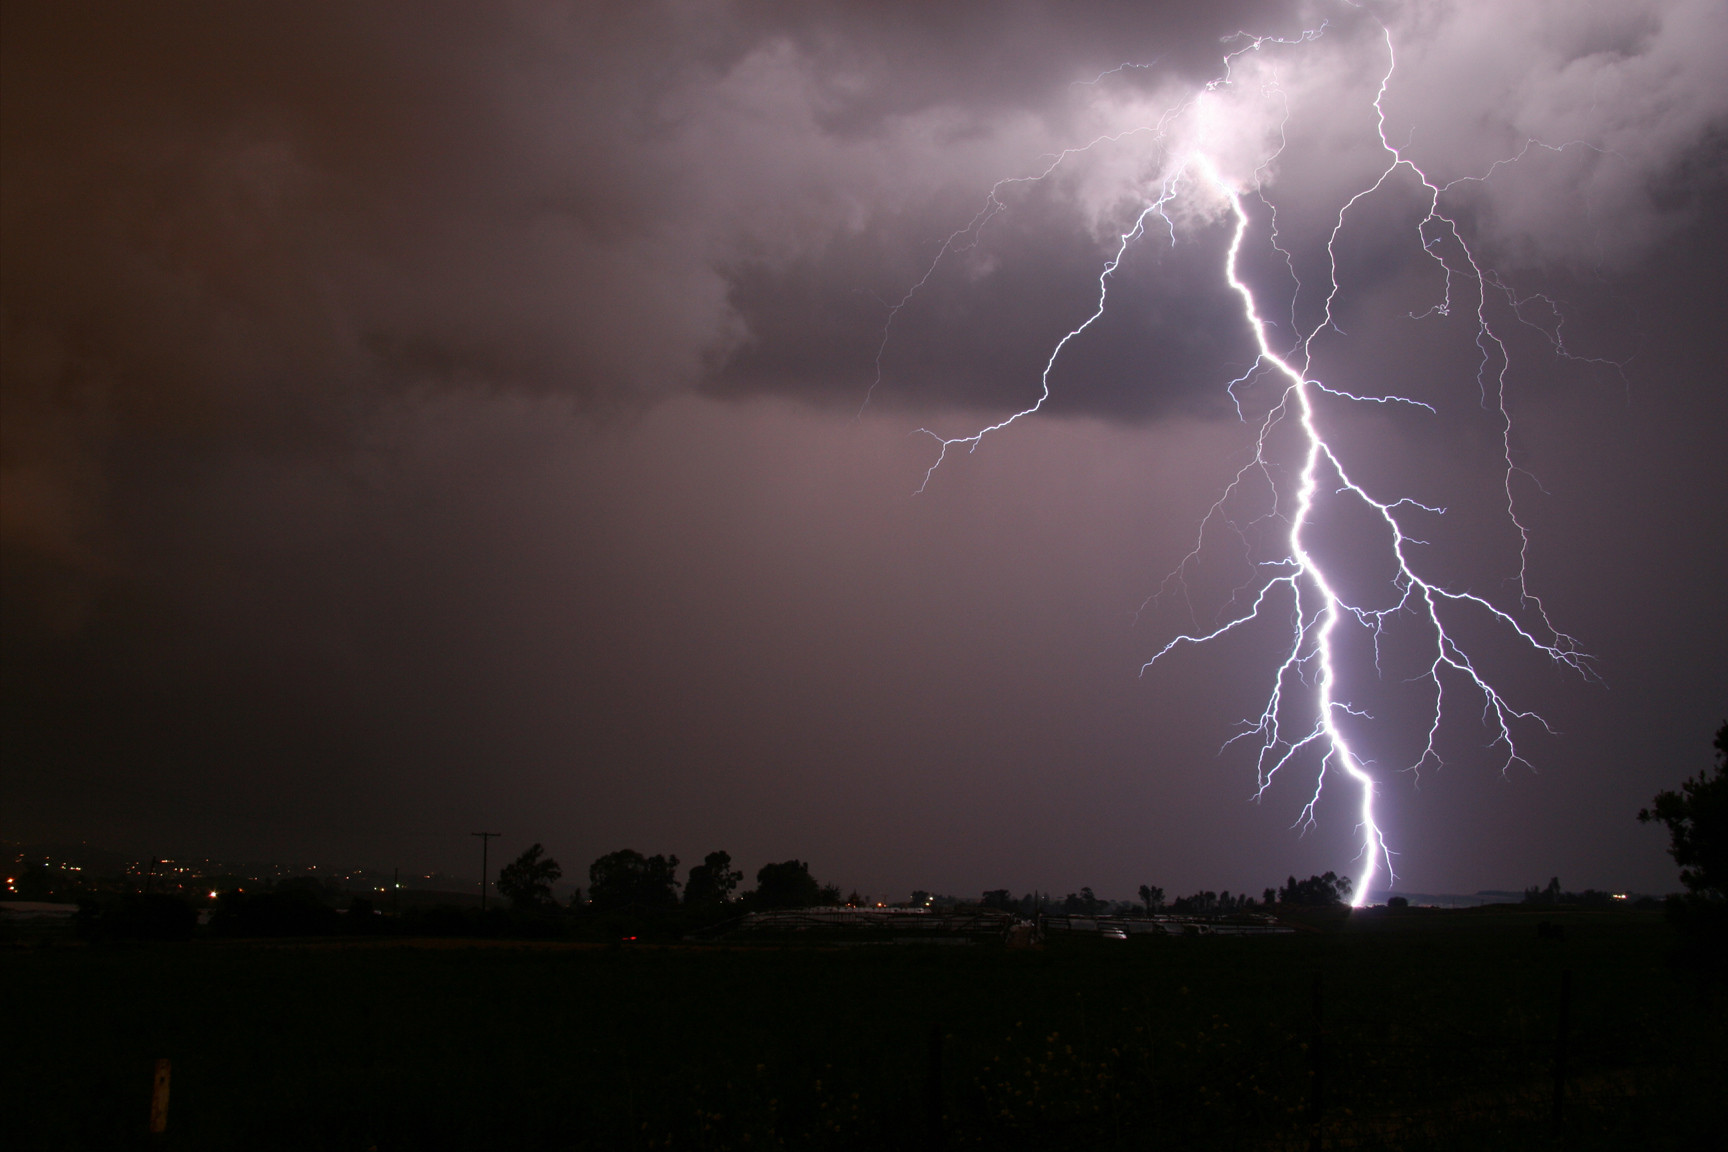
\includegraphics[
    	% width=\paperwidth,
    	height=1.05\paperheight
    	]{light}};
    
    %\fill[color=base](0.4,7.8cm) rectangle(9cm, 7.15cm);    
    %\fill[color=base](1.3cm,4.2cm) rectangle(5.5cm,3.8cm);
    %\fill[color=base](1.1cm,3.2cm) rectangle(6.3cm,2.8cm);
    %
    % muda
    % 
    %%		
    \node[anchor=north east] at (12.8cm,9.6cm){
\includegraphics[height=11mm]{logoicexbrancosharp}};
    \node[anchor=north west] at (.2cm,9.6cm){
\includegraphics[height=11mm]{logoUFF}};
    %%		% draw the actual text
    \node[anchor=south,text width=11.8cm,inner xsep=0.5cm] at (6.8cm,6cm) {\color{white}{\Huge\firaheavy{\inserttitle}}};
    \node[anchor=north east,text width=11.8cm, align=center] at (9.5cm,6cm) {\color{white}\Large\insertsubtitle};
    \node at (3.4cm,4cm) {\color{white}\LARGE\textsc{\firasemibold\insertauthor}};
    \node at (3.4cm,3cm) {\color{white}\large\firalight\insertinstitute};
    
    %		
    %		% add the date in the corner
    \node[anchor=south east] at(12.8cm,0cm) {\color{base}\tiny\insertdate};	
    \else
    %	
    %	% the background
    \fill[color=white] (0,0) rectangle(12.8cm,9.6cm);
    % separate the drawing based on if we're the first (title) slide or not
    % not the title page
    % title bar
    %\fill[color=base] (0, 8.6cm) rectangle(12.8cm,9.6cm);
    % swap the comment on these to add section titles to slide titles
    %\node[anchor=north,text width=11.8cm,inner xsep=0.5cm,inner ysep=0.25cm] at (6.4cm,9.6cm) {\color{white}\Large\textbf{\insertsectionhead: \insertframetitle}};
    %\node[anchor=north,text width=11.8cm,inner xsep=0.5cm,inner ysep=0.25cm] at (6.4cm,9.6cm) {\color{white}\huge\textbf{\insertframetitle}};
    % if we're showing a progress bar, show it
    % (I disable the progress bar and slide numbers for the "Appendix" slides)
    \ifnum \value{showProgressBar}>0\relax%
    % the the progress bar icon in the middle of the screen
    %\draw[fill=grey,draw=none] (0cm,0.25cm) rectangle(12.8cm
    %,0.23cm);
    \draw[fill=base,draw=none] (0cm,0.27cm) rectangle(\progressbar@tmpdim,0.26cm);
    
    % bottom information
    \node[anchor=south west] at(0cm,-0.1cm) {\color{base}\tiny\textbf{\insertsection}\;  \insertsubsectionhead};
    % if slide numbers are active
    \ifnum \value{showSlideNumbers}>0\relax%
    % if slide totals are active
    \ifnum \value{showSlideTotal}>0\relax%
    % draw both slide number and slide total
    \node[anchor=south east] at(12.8cm,-0.10cm) {\color{black}\tiny\insertframenumber/\inserttotalframenumber
    	%\inserttotalframenumber
    	};
    \else
    % slide totals aren't active, don't draw them
    \node[anchor=south east] at(12.8cm,0.25cm) {\color{grey}\tiny\insertframenumber};
    \fi
    \fi			
    % don't show the progress bar?
    \else
    % section title in the bottom left
    \node[anchor=south west] at(0cm,0cm) {\color{grey}\tiny\insertsection};
    % if we're showing slide numbers
    \ifnum \value{showSlideNumbers}>0\relax%
    % if slide totals are active
    \ifnum \value{showSlideTotal}>0\relax%
    % draw both slide number and slide total
    \node[anchor=south east] at(12.8cm,0cm) {\color{grey}\tiny\insertframenumber/\inserttotalframenumber};
    \else
    % slide totals aren't active, don't draw them
    \node[anchor=south east] at(12.8cm,0cm) {\color{grey}\tiny\insertframenumber};
    \fi
    \fi
    \fi			
    \fi
    \end{tikzpicture}
}
\makeatother			

%% use a small dash ('-') for a bulletpoint list
%\setbeamertemplate{itemize %item}{\usebeamercolor[fg]{item}\small\ECFAugie{*}}

%%% Frametitle
\setbeamertemplate{frametitle}{
    \nointerlineskip
    \begin{beamercolorbox}[wd=\paperwidth,ht=0.8cm,dp=0ex]{frametitle}
        \usebeamerfont{frametitle}
        \strut\insertframetitle\strut \hfill \\
        %\raisebox{-1mm}{\includegraphics[height=0.6cm]{logoicexbranco}}\\  
    \end{beamercolorbox}
}

%% remove navigation symbols
\setbeamertemplate{navigation symbols}{}

%\AtBeginSection[]
%{ 
%	\begin{frame}{Sumário}
%	\small{\tableofcontents[currentsection,currentsubsection]}
%	\end{frame}
%} 

\AtBeginSection{\frame[noframenumbering]{\sectionpage}}
\setbeamertemplate{section page}
{
	\sloppy
	\transboxout
    
\begin{tikzpicture}
    % set up the entire slide as the canvas
    \useasboundingbox (0,0) rectangle(\the\paperwidth,\the\paperheight);
    %\fill[color=white] (-1cm, 1cm) rectangle(11.8cm, 9.8cm);
    \fill[color=base] (-1cm, 0cm) rectangle(11.8cm, 9.8cm);
    \node[text width=11cm,align=center] at (5.4cm, 4.9cm) {\color{white}\Huge\textbf{\insertsection}};
    \end{tikzpicture}
}

\AtBeginSubsection{\frame[noframenumbering]{\subsectionpage}}
\setbeamertemplate{subsection page}
{   \transboxout
	
\begin{tikzpicture}
	% set up the entire slide as the canvas
	\useasboundingbox (0,0) rectangle(\the\paperwidth,\the\paperheight);
	%\fill[color=white] (-1cm, 1cm) rectangle(11.8cm, 9.8cm);
	\fill[color=base] (-1cm, 0cm) rectangle(11.8cm, 9.8cm);
	\node[text width=11.8cm,align=center] at (5.4cm, 4.9cm) {\color{white}\Huge\textbf{\insertsubsection}};
	\end{tikzpicture}
}



\setbeamertemplate{section in toc}[sections numbered]
\setbeamertemplate{subsection in toc}[subsections numbered]
\setbeamercolor{block body}{bg=black!8}
\DeclareMathOperator{\sen}{sen}
\newcommand{\ddt}[2]{\ensuremath\dfrac{d#1}{d#2}}
\newcommand{\ddtp}[2]{\ensuremath\frac{\partial #1}{\partial #2}}
\newcommand{\titulo}[1]{\textbf{\Large\textsc{\color{base}#1}}}

%
%   Dados do curso
% muda
\title{Git: mantendo versões}
\subtitle{e sua sanidade mental}
\author{Thadeu Penna}
\date{\today}
\institute{thadeupenna@id.uff.br}
\pgfplotsset{compat=1.12}



\sisetup{output-decimal-marker = {,}}
\newcommand{\meio}{\nicefrac{1}{2}}
\definecolor{deepblue}{rgb}{0,0,0.5}
\definecolor{deepred}{rgb}{0.6,0,0}
\definecolor{deepgreen}{rgb}{0,0.5,0}
\DeclareFixedFont{\ttb}{T1}{txtt}{bx}{n}{7} % for bold
\DeclareFixedFont{\ttm}{T1}{txtt}{m}{n}{7}  % for normal

\newcommand\pythonstyle{\lstset{
		language=Python,
		basicstyle=\scriptsize,
		otherkeywords={typeof, null, catch, switch, in, int, str, float, self},
		ndkeywords={boolean, throw, import},
		ndkeywords={return, class, if ,elif, endif, while, do, else, True, False ,  catch, def},
		ndkeywordstyle=\color{BrickRed},
		identifierstyle=\color{deepblue},
		sensitive=false,
		otherkeywords={self},             % Add keywords here
		keywordstyle=\color{deepgreen},
		emph={MyClass,__init__},          % Custom highlighting
		emphstyle=\color{deepred},    % Custom highlighting style
		stringstyle=\color{deepgreen},
		commentstyle=\color{red},
		tabsize=4,
		frame=tb,                         % Any extra options here
		showstringspaces=false            % 
}}
	
% Python environment
\lstnewenvironment{python}[1][]
{
\pythonstyle
\lstset{#1}
}
{}
	
% Python for external files
\newcommand\pythonexternal[2][]{{
\pythonstyle
\lstinputlisting[#1]{#2}}}
	
% Python for inline
\newcommand\pythoninline[1]{{\pythonstyle\lstinline!#1!}}


\definecolor{mGreen}{rgb}{0,0.6,0}
\definecolor{mGray}{rgb}{0.5,0.5,0.5}
\definecolor{mPurple}{rgb}{0.58,0,0.82}
\definecolor{backgroundColour}{rgb}{1,1,1}

\lstdefinestyle{cstyle}{
	backgroundcolor=\color{backgroundColour},   
	commentstyle=\color{mGreen},
	keywordstyle=\color{magenta},
	numberstyle=\tiny\color{mGray},
	stringstyle=\color{mPurple}\ttfamily,
%    basicstyle=\ttfamily,
%    keywordstyle=\color{blue},
%    stringstyle=\color{red},
%    commentstyle=\color{green},
%    morecomment=[l][\color{magenta}]{\#}
	basicstyle=\small\ttfamily,
	breakatwhitespace=false,         
	breaklines=true,                 
	captionpos=b,                    
	keepspaces=true,                 
	numbers=left,  
	numberstyle=\tiny,                  
	numbersep=5pt,                  
	showspaces=false,                
	showstringspaces=false,
	showtabs=false,                  
	tabsize=2,
	language=C
}



\newcommand{\nocanto}{\vspace{-0.13cm}\hspace*{-1.2cm}}

\newenvironment{terminal}[1]{
\noindent  \renewcommand\arraystretch{0.85}
\begin{alertblock}{\hfill #1 \hfill -\;+\;x}
}{
\end{alertblock}}

\setbeamertemplate{itemize item}{
	%\MVRightarrow
	\faArrowRight
	%\raise-2pt\hbox{\includegraphics[height=0.4cm]{right.jpg}}
	}

\lstset{
	literate={ö}{{\"o}}1
	{ô}{{\^o}}1
	{ü}{{\"u}}1
}

\begin{document}
\tikzstyle{every picture}+=[remember picture]

	\begin{frame}
		\transfade
		\titlepage
	\end{frame}

\newenvironment{amatrix}[1]{%
	\left(\begin{array}{@{}*{#1}{c}|c@{}}
	}{%
\end{array}\right)
}

\begin{frame}{Sumário}
\tableofcontents
\end{frame}
\section{Motivação}
\begin{frame}{Acabou de Aprender uma linguagem de Programação}
	\nocanto
\includegraphics[width=1.02\paperwidth,height=0.92\paperheight]{../figures/prog1}
\end{frame}

\begin{frame}{Fases do Desenvolvimento}
	\nocanto\vspace{-0.5cm}
	\begin{center}
		
\includegraphics[width=0.7\paperwidth]{programafases}
	\end{center}
\end{frame}

\begin{frame}{Caça aos bugs}
	\nocanto
\includegraphics[width=1.22\paperwidth]{bughunter}
\end{frame}

\subsection{Lição 1:\break Debugar é ruim.\break Testar é legal.}
\begin{frame}{TDD: Test Driven Development}
	\nocanto\vspace{-0.5cm}\begin{center}
		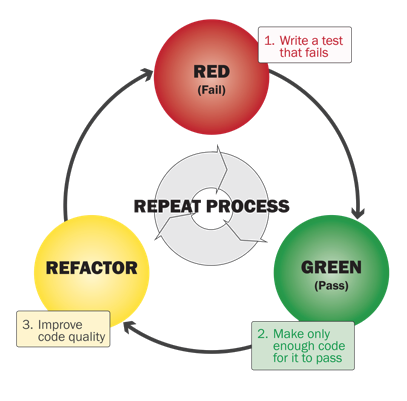
\includegraphics[height=.9\paperheight]{tdd}
	\end{center}
\end{frame}

\begin{frame}{TDD: Mudar o Código sem Medo de Causar Desastres}
	\nocanto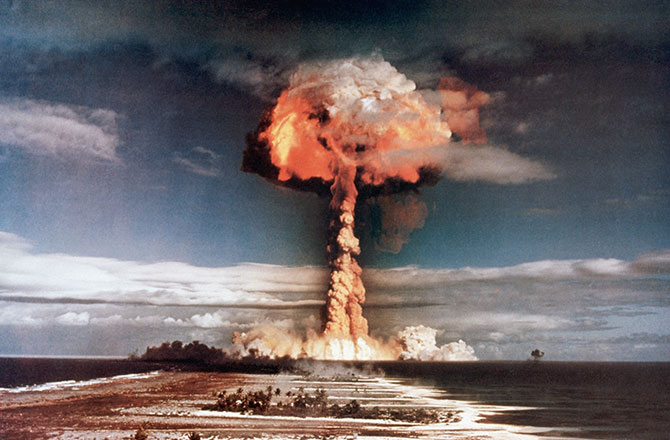
\includegraphics[width=1.03\paperwidth]{nuclearbomb}
\end{frame}

\begin{frame}{TDD: Baby Steps}
	\nocanto
\includegraphics[width=1.03\paperwidth]{baby-steps}
\end{frame}

\subsection{Análise de um chute}
\begin{frame}{Folha Seca do Zico}
	\begin{center}
		\movie[autostart,
		height=0.7\textheight,
		width=\textwidth,
		showcontrols,
		poster
		]{}{zico.mp4}
	\end{center}
	%    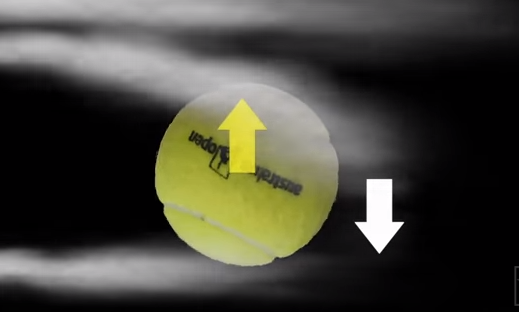
\includegraphics[width=\textwidth]{magnus}
\end{frame}

\begin{frame}{Exemplo: Simular a bola em um chute}
	
\begin{enumerate}
	\item Do que depende ?\\
	velocidade inicial, ângulo(s), vento, gravidade, rotação (efeito)
	\item Como atualizo ? \\
	função para mover a bola. Testo se em $t\neq 0$, $x\neq 0$.
	\item Move na horizontal ? \\
	Veja se $x=vt$
	\item Move na vertical ? \\
	Veja se $y\neq 0$
	\item Como descubro o alcance ? \\
	Veja se $y=0$ se $\theta=90^o$. $45^o$ é máximo ?
	\item adiciono 3D. Testa $x-y$, $x-z$, etc.
	\item adiciono o vento. Testa se aumenta o alcance
	\item adiciono a rotação da bola. Testo a movimentação. 
\end{enumerate} 	
\end{frame}

\section{Git Yourself:\break Git do Eu Sozinho}
\begin{frame}{Controle de Versões}
	
Mais usado: Nenhum controle. Você pode facilmente destruir um programa que funcionava antes.	

\begin{center}
	
\includegraphics[width=0.8\textwidth]{disgirl}
\end{center}
\end{frame}

\subsection{Diff e Patch}
\begin{frame}[fragile]{diff e patch: os primórdios}
Escreva um programa que imprima \ttblue{''Hello, world!''} na tela.

\begin{lstlisting}[style=cstyle]
#include <stdio.h>

int main() {
	printf("Hello, world!\n");	
}
\end{lstlisting}
Salve o arquivo como \texttt{hello.c}\\
Altere o programa para escrever ``Alô, mundo'' e salve como \texttt{hello2.c}  (pode fazer o mesmo em qualquer linguagem). Rode
\begin{terminal}{\~}
\begin{Verbatim}
$ diff hello.c hello2.c
4c4
<    printf("Hello, world!\n");	
---
>    printf("Alô, mundo!\n");	
\end{Verbatim}
\end{terminal} 
\end{frame}

\begin{frame}[fragile]{diff -uNr}
\begin{terminal}{\~}
\begin{Verbatim}
$ diff -uNr hello.c hello2.c 
--- hello.c	2017-10-23 18:33:35.945704069 -0200
+++ hello2.c	2017-10-23 18:33:59.881753109 -0200
@@ -1,5 +1,5 @@
#include <stdio.h>

int main() {
-   printf("Hello, world!\n");	
+   printf("Alô, mundo!\n");	
}
\end{Verbatim}
\end{terminal}
\texttt{diff} funciona entre diretórios também. 
\begin{itemize}
	\item \texttt{-u}: cria cabeçalho e linhas próximas
	\item \texttt{-N}: arquivos inexistentes como vazios
	\item \texttt{-r}: recursivo, i.e., procura dentro de diretórios. 
	\item \texttt{diff --help} para mais opções
\end{itemize}
\end{frame}

\begin{frame}[fragile]{Patch}
\begin{terminal}{\~}
\begin{Verbatim}	
$ cat hello.c
$ diff -uNr hello.c hello2.c > hello.patch
$ patch -p1 hello.c < hello.patch
$ cat hello.c 
\end{Verbatim}
\end{terminal}
\begin{itemize}
	\item \texttt{-b}: faz backup do original
\end{itemize}
É possível manter a história de todas as versões usando \texttt{patch} e \texttt{diff}. É possível mas não é divertido.
\vfill
Imagine se pudesse ter apenas o arquivo da versão mais atual na sua vista, mas pudesse acessar as anteriores quando quisesse. Para isso, existe o \texttt{git} (mas não só para isso).
\vfill
\end{frame}

\subsection{VCS}
\begin{frame}{VCS}
	\textbf{VCS:} version control system. Gerenciar as mudanças que acontecem nos seus programas. É fundamental para grandes projetos, com colaborações, mas ajuda mesmo em pequenos códigos. Exemplos: CVS, SVN, Mercurial, BitKeeper e Git. 
\end{frame}

\begin{frame}{Git}
\begin{itemize}
	\item Criado por Linus Torvalds, em 2005. 
	\item Manutenção do kernel Linux
	\item Hoje: 19.786.000 linhas de código
	\item Mais de 2000 contribuidores ativos (Linus contribui com menos de 0,3\% do código). 15 mil no total.
	\item BitKeeper fechou o código 
	\item Pode ser usado sem conexão de rede.  
\end{itemize}	
\end{frame}

\begin{frame}{Modelos}
	\centering
	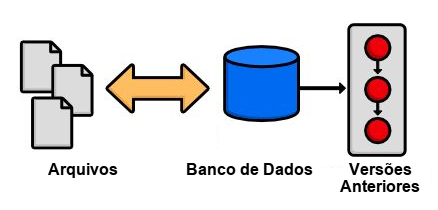
\includegraphics[width=0.4\textwidth]{vcslocal}\\
	Local
	\begin{columns}
		\begin{column}{0.45\textwidth}
		   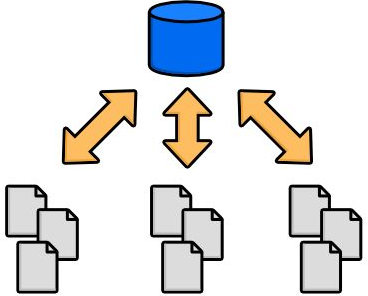
\includegraphics[width=\textwidth]{vcscentr}\\Centralizado: conflitos / merge 
		\end{column}
		\begin{column}{0.45\textwidth}
			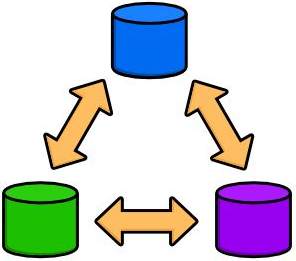
\includegraphics[width=\textwidth]{vcsdist}\\
			Distribuído 
			\end{column}
	\end{columns}
\end{frame}

\subsection{Git na Prática}
\begin{frame}[fragile]{Inicializando o Git}
Desenvolvido em 2005, pelo Linus Torvalds. O kernel Linux tem cerca de 20 milhões de linhas de código, mantido por 15 mil colaboradores. 
\begin{terminal}{Terminal}
\begin{Verbatim}[fontseries=b]
$ mkdir Hello
$ cd Hello
$ git init
 Initialized empty Git repository in ... 
$ ls -a
 .  ..  .git
$ git status

$ git config --global user.name "Thadeu Penna"
$ git config --global user.email thadeupenna@id.uff.br
$ git config --global core.editor vim
\end{Verbatim}
\end{terminal}
Use \texttt{vim},~\texttt{nano},~\texttt{gedit}, etc.\\
Os comandos \texttt{git config} configuram o \texttt{git} globalmente, isto é, valem para outros repositórios a serem criados.
\end{frame}


\subsection{Modificando o Código e Salvando as Versões}
\begin{frame}[fragile]{Adicionando arquivos}
Crie um arquivo \ttblue{hello.c} ou copie o arquivo anterior para este diretório. 
\begin{terminal}{Terminal}
\begin{Verbatim}[fontseries=b]
$ git status
$ git add hello.c
$ git status 
No ramo master

Submissão inicial.
Mudanças a serem submetidas:
(utilize "git rm --cached <arquivo>..." para não apresentar)

new file:   hello.c

$ git log
fatal: your current branch 'master' does not have any 
commits yet
\end{Verbatim}
\end{terminal}
\end{frame}	

\begin{frame}{Os Estágios do Git}
\begin{center}
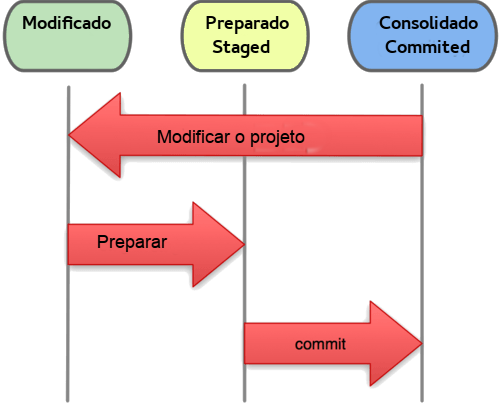
\includegraphics[width=\textwidth, height=0.8\textheight]{gitestados}
\end{center}	
\end{frame}

\begin{frame}[fragile]{O Primeiro Commit}
\begin{terminal}{Terminal}
\begin{Verbatim}[fontseries=b]
$ git status
$ git commit -m "Criação do arquivo"
[master (root-commit) 9df8c85] Criação do arquivo
1 file changed, 5 insertions(+)
create mode 100644 hello.c
$ git status
$ git log
$ git log --oneline
\end{Verbatim}
\end{terminal}
\begin{center}
	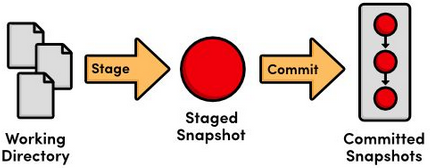
\includegraphics[width=0.5\textwidth]{commit}
\end{center}	
\end{frame}
%
%
\begin{frame}[fragile]{O Segundo Commit}
	Altere o arquivo \texttt{hello.c} para escrever em português. Salve o arquivo. 
	\begin{terminal}{Terminal}
		\begin{Verbatim}[fontseries=b]
$ git status
Changes not staged for commit:
modified:   hello.c
$ git add hello.c
$ git status
(use "git reset HEAD <file>..." to unstage)
	  modified:   hello.c
$ git commit -m “Traduzido para o português”
[master 27be570] Traduzido para o Português
 1 file changed, 1 insertion(+), 1 deletion(-)
$ git log --oneline
27be570 Traduzido para o Português
9df8c85 Criação do arquivo
\end{Verbatim}
\end{terminal}
\end{frame}

\begin{frame}[fragile]{Git Checkout}
Temos dois commits até agora (os números serão diferentes em cada máquina). O arquivo \texttt{hello.c} contém a versão em português. Verifique as saídas dos comandos 
\begin{terminal}{Terminal}
\begin{Verbatim}[fontseries=b]
$ git log --oneline
27be570 Traduzido para o Português
9df8c85 Criação do arquivo
$ git checkout 9df8c85 
HEAD is now at 9df8c85... Criação do arquivo

$ cat hello.c
$ git log --oneline
\end{Verbatim}
\end{terminal}
O que aconteceu com o \texttt{hello.c} ? \\ 
Observem o aviso. O \texttt{git} é bem pedagógico. O HEAD está agora no primeiro commit. HEAD é a posição atual do sistema modificado e o master é o do último commit. 
\end{frame}

\begin{frame}[fragile]{Git Checkout}
Verifique as saídas dos comandos 
\begin{terminal}{Terminal}
\begin{Verbatim}[fontseries=b]
$ git status
HEAD detached at 9df8c85
nada a submeter, diretório de trabalho vazio
$ git checkout master
Previous HEAD position was 9df8c85... Criação do arquivo
Switched to branch 'master'
$ cat hello.c
\end{Verbatim}
\end{terminal}
\end{frame}

\begin{frame}{Entendendo o Git}
	\only{Visão Tradicional}<1>
	\only{Visão do Git, snapshots}<2>
	\begin{overprint}
		\includegraphics<1>[width=\textwidth]{gitway1}
		\includegraphics<2>[width=\textwidth]{gitway2}
	\end{overprint}
\end{frame}

\begin{frame}[fragile]{Git Diff - O que mudou ? }
Suponha que agora você queira ver as diferenças entre dois checkouts. 
\begin{terminal}{Terminal}
\begin{Verbatim}[fontseries=b]
$ git log --oneline 
27be570 Traduzido para o Português
9df8c85 Criação do arquivo
$ git status
No ramo master
$ git diff 9df8c85 
--- a/hello.c
+++ b/hello.c
@@ -1,5 +1,5 @@
#include <stdio.h>

int main() {
-   printf("Hello, world!\n");     
+   printf("Alô, mundo!\n");    
\end{Verbatim}
\end{terminal}
\end{frame}


\begin{frame}[fragile,allowframebreaks]{Revertendo Commits}
\begin{itemize}
\item Se você esqueceu de adicionar um arquivo no último commit
\begin{terminal}{\~}
\begin{Verbatim}[fontseries=b]
$ git add outroarquivo.dat
$ git commit --amend
\end{Verbatim}
\end{terminal}
\item Você acabou de modificar o arquivo, mas se arrependeu.  	
\begin{terminal}{\~}
\begin{Verbatim}[fontseries=b]
$ git status  
(utilize "git add <arquivo>..." para atualizar 
o que será submetido)
(utilize "git checkout -- <arquivo>..." para descartar
mudanças no diretório de trabalho)

modified:   hello.c
$ git checkout -- hello.c
\end{Verbatim}
\end{terminal}
\item Você se arrependeu do último commit  	
\begin{terminal}{\~}
\begin{Verbatim}[fontseries=b]
$ git log --oneline
f950da4 Vírgula
...
$ git revert f950da4 
\end{Verbatim}
\end{terminal}
\item Adicionou um arquivo para o staged e se arrependeu
\begin{terminal}{\~}
\begin{Verbatim}[fontseries=b]
$ git add dados.dat
$ git status
Mudanças a serem submetidas:
  (use "git reset HEAD <file>..." to unstage)
  
  new file:   dados.dat
  	
$ git reset HEAD dados.dat
\end{Verbatim}
\end{terminal}
\end{itemize}	
\end{frame}
	
\begin{frame}[fragile]{Etiquetando os commits}
\begin{terminal}{\~}
\begin{Verbatim}[fontseries=b]
$ git tag -a v1.0 -m "Versão estável"
$ git status 
$ git checkout -a v1.0
\end{Verbatim}
\end{terminal}
\end{frame}	

\begin{frame}[allowframebreaks]{Cheatsheet}
	\begin{description}[labelwidth=\widthof{\bfseries git -am xxx }]
		\item[git config -{}-global -{}-list ] Lista configurações globais
		\item[git status -s] Status resumido(silent) 
		\item[git add .] Adiciona todo o diretório
		\item[git commit -a -m “ok”] Adiciona e faz o commit
		\item[git rm dados.dat] Remove dados.dat do git e do diretório
		\item[git clean -f] Limpa arquivos modificados
		\item[git clean -n] Mostra o que vai ser apagado
		\item[git log -p] Mostra as mudanças 
		\item[git tag -l -n1] Versões e mensagens
		\item[.gitignore] Arquivo com especificações para ignorar arquivos (*.o, *.aux, por exemplo). Um tipo por linha.
		\item[git help] O mais útil deles  
		\item[\url{http://git-scm.com}] Documentação sobre o Git.
	\end{description}
\end{frame}

\subsection{Resumo}
\begin{frame}{WorkFlow}
\begin{enumerate}
	\item Cria diretório
	\item \ttblue{git init}
	\item \ttblue{git add}
	\item \ttblue{git commit -m ””}
	\item \ttblue{git status}
	\item \ttblue{git log}
\end{enumerate}	
\end{frame}


\subsection{Branches}
\begin{frame}{Branches}
	Branch é um ramo independente de desenvolvimento. Imagine que duas pessoas tenham que mexer no código, mas criando funções independentes. Cada uma cria um branch e depois os mesmos são ligados ao tronco principal, o \ttblue{master}. Ou mesmo, você quer tentar duas saídas diferentes para um mesmo problema mas não está certo de que escolha será a melhor. Se não der certo, voltamos ao programa original. 
	\vfill
	Aqui é que reside o grande poder de organização do \texttt{git}. A página inicial do curso tem um relâmpago com branches, para ressaltar a importância deste procedimento. 
	\vfill
\end{frame}

\begin{frame}[fragile]{Criando um branch}
Imagine que você tenha criado um arquivo e “commitado” algumas modificações. 
\begin{center}
	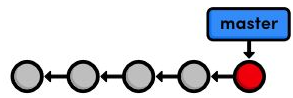
\includegraphics[width=0.3\textwidth]{master}
\end{center}
O nosso programa já imprime \ttblue{“Alô, mundo!”}.
Vamos criar um branch para imprimir os números pares, mas você não quer perder o que já funciona tão bem.  
\begin{terminal}{Terminal}
\begin{Verbatim}[fontseries=b]
$ git branch
* master
$ git branch pares
$ git branch
  pares
* master
$ git checkout pares
Switched to branch 'pares'
\end{Verbatim} 
\end{terminal}
\end{frame}

\begin{frame}[fragile]{Modificando um Branch}
No momento estamos assim:
\begin{center}
		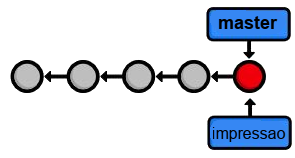
\includegraphics[width=0.35\textwidth]{branchi}
\end{center}

\begin{lstlisting}[style=cstyle]
#include <stdio.h>

void main() {
int i;

printf("Oi Mundo!\n");	
for (i=0;i<=10;i+=2) printf("%d\n",i);
}

\end{lstlisting}
\end{frame}

\begin{frame}[fragile]{Modificando no Branch}
\begin{terminal}{\~}
\begin{Verbatim}[fontseries=b]
$ git commit -m "Imprime pares"
$ git log --oneline
9488aec Imprime pares
27be570 Traduzido para o Português
.... 
$ git branch
* pares
master
$ git checkout  master
Switched to branch 'master'
$ git log --oneline
27be570 Traduzido para o Português
....
\end{Verbatim}
Observe que, no master, não há referência ao que aconteceu no branch pares. 
\end{terminal}	
\end{frame}
%
\begin{frame}[fragile]{Merge}
Se o programa funcionar, é hora de adicionar a modificação ao master.
\begin{terminal}{Terminal}
\begin{Verbatim}[fontseries=b]
$ git branch
pares
* master 
$ git merge pares
Updating d054ccd..9488aec
Fast-forward
hello.c | 5 ++++-
1 file changed, 4 insertions(+), 1 deletion(-)
$ git status
No ramo master
nada a submeter, diretório de trabalho vazio
$ git log --oneline --decorate --all --graph 
\end{Verbatim} 
\end{terminal}	
\end{frame}

\begin{frame}[fragile]{Fast-Forward Merge}
	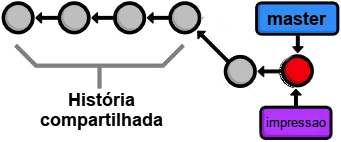
\includegraphics[width=0.6\textwidth]{branch3i}
	\begin{terminal}{Terminal}
		\begin{Verbatim}[fontseries=b]
$ git branch -d impressao
Deleted branch impressao (was 79628c5).
$ git branch
* master
		\end{Verbatim}
	\end{terminal}
\end{frame}

\begin{frame}[fragile]{Entendendo o Merge}
	Use o \texttt{git revert } para voltar a versão sem impressão dos pares. Crie dois branches (par e impar), um para mostrar os pares e outro para mostrar os ímpares.
	
	O que daria o merge de um e depois o outro ?  

\begin{lstlisting}[style=cstyle]
#include <stdio.h>

void main() {
  int i;

  printf("Oi Mundo!\n");	
  for (i=0;i<=10;i+=2) printf("%d\n",i);
}

\end{lstlisting}
	
\end{frame}

\begin{frame}[fragile]{Entendendo o Merge}
	Use o \texttt{git revert } para voltar a versão sem impressão dos pares. Crie dois branches (par e impar), um para mostrar os pares e outro para mostrar os ímpares, através de uma função.
	
	O que daria o merge de um e depois o outro ?  
	
\begin{lstlisting}[style=cstyle]
#include <stdio.h>

void imprime_pares(int n) {
	int i;

	for(i=0;i<=n;i+=2) printf("%d\n",i); 
}

void main() {
	printf("Alô Mundo!\n");
	imprime_pares(10);
}
\end{lstlisting}
\end{frame}

\begin{frame}{3-way Merge}
%	Imagine que você precisa fazer duas alterações no código: por exemplo, mudar a dimensão da matriz e imprimir o vetor com os resultados. São duas alterações simples, mas vamos usar o git para isso. Faça os seguintes passos, na ordem: 
%	\begin{enumerate}
%		\item Crie o branch phase.
%		\item Vá para o branch phase. Modifique o programa para imprimir um vetor. Faça o commit.
%		\item Vá para o branch master, mude a dimensão da matriz. Faça o commit. 
%	\end{enumerate}
	\begin{center}
		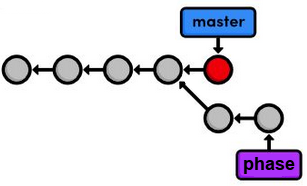
\includegraphics[width=0.45\textwidth]{3way-1}
	\end{center}
\end{frame}
%
\begin{frame}{3-way Merge}
	\begin{center}
		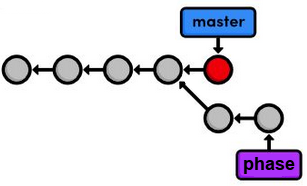
\includegraphics[width=0.45\textwidth]{3way-1}\\
		\hrulefill \\
		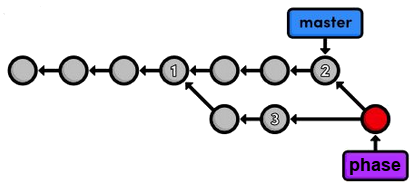
\includegraphics[width=0.6\textwidth]{3way-2}
	\end{center}
%	Tente fazer o merge. O que aconteceu ?
\end{frame}

\begin{frame}[fragile]{Resolvendo Conflitos}
\begin{terminal}{Terminal}
\begin{Verbatim}[fontseries=b]
$ git merge impar
Mesclagem automática de sistemas.c
CONFLITO (conteúdo): conflito de mesclagem em hello.c
Automatic merge failed; fix conflicts and then commit
the result.
\end{Verbatim}
\end{terminal}

	Abra o arquivo e encontre o local de conflito.\\ \textbf{Sim, mensagens de erro devem ser lidas cuidadosamente}. \\
	Edite-o, adicione-o e faça o novo commit.
\end{frame}

\begin{frame}[fragile]{Comandos Úteis para Arquivar}
	\begin{description}
		\item[\color{red}\ttblue{git archive master --format=zip -o ../backup.zip}]
		\item[\color{red}\ttblue{git archive master -o ../backup.tar.gz}] Copia todos os arquivos do ramo master. Não copiará a informação do git. 				
		\item[\color{red}\ttblue{git bundle create repo.bundle master}]  Cria um arquivo repo.bundle, incluindo as informações do .git. 
		\item[\color{red}\ttblue{git clone repo.bundle outrolugar -b master}] Recria toda a árvore do git, salva em repo.bundle, no diretório outrolugar.		
	\end{description}
\end{frame}		

\section{GitHub\break Eu e você, a dois, a três, escancarando de vez }

\begin{frame}{GitHub}
	\vfill
	O GitHub \url{https://github.com} é o repositório mais usado para manter projetos open-source. Outro site interessante é o Bitbucket \url{https://bitbucket.org/}. Você pode hospedar seus projetos lá, sem custos, desde que os projetos sejam abertos. O BitBucket permite hospedagem de projetos privados gratuitamente também. 
	\vfill
	É possível rodar o git em um diretório compartilhado, tipo Google Drive ou Dropbox, podendo acessá-lo a partir de máquinas diferentes. O GitHub vai além disse, facilitando colaborações.
	\vfill
\end{frame}

\begin{frame}{GitHub}
	\nocanto
	
\includegraphics[width=1.03\paperwidth]{githubhome}
\end{frame}

\begin{frame}{GitHub}
	\vspace{-0.12cm}\hspace*{-0.9cm}
	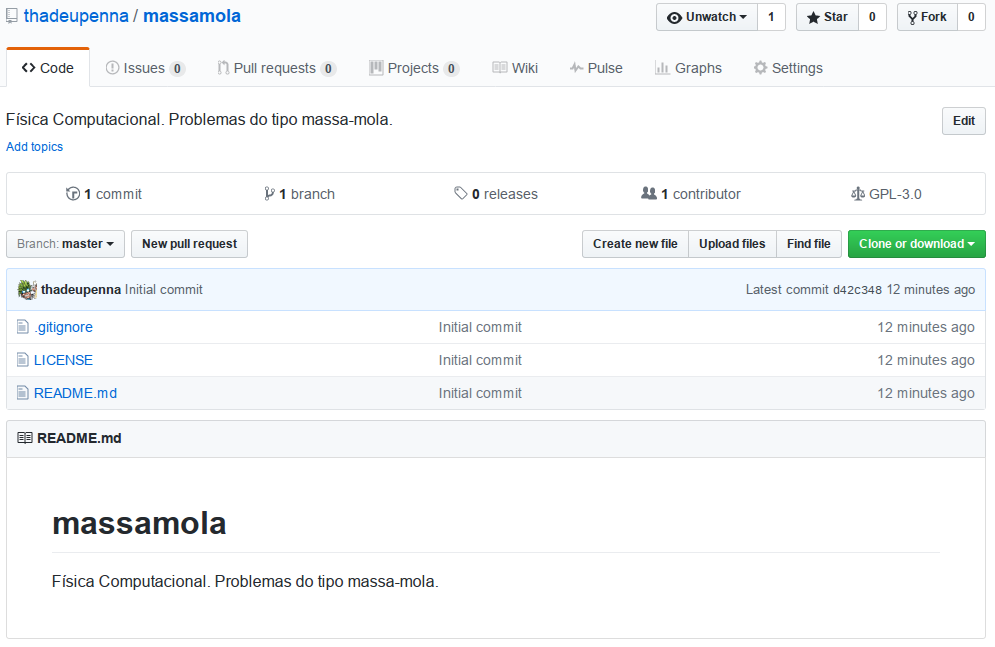
\includegraphics[width=0.9\paperwidth]{github2}
\end{frame}

\begin{frame}[fragile]{Markdown}
	\url{https://guides.github.com/features/mastering-markdown}
	
\begin{description}
\item[\bf Seções] \hfill\\
\begin{Verbatim}
# This is an <h1> tag
## This is an <h2> tag
###### This is an <h6> tag
\end{Verbatim}
\item[\bf Fontes] \hfill \\
\begin{Verbatim}
It's very easy to make some words **bold** 
and other words *italic* with Markdown. 
You can even [link to Google!](http://google.com)
\end{Verbatim}
\item[\bf Imagens] \hfill \\
\begin{Verbatim}
![GitHub Logo](/images/logo.png)
Format: ![Alt Text](url)
\end{Verbatim}
\end{description}
\end{frame}
%

\begin{frame}[fragile]{Atualização}
	
	URL é do tipo \url{https://github.com/thadeupenna/massamola.git}
	
{\Large Muito Fácil}
\begin{terminal}{Terminal}
\begin{Verbatim}[fontseries=b]
$ git remote add origin URL 
$ git clone URL 

$ git pull origin master
warning: no common commits
remote: Counting objects: 5, done.

$ git push  -u origin master
Counting objects: 36, done.
\end{Verbatim}		
\end{terminal}
\begin{description}
\item[\color{red}pull] pega do github
\item[\color{red}push] joga no github
\end{description}
\end{frame}


\begin{frame}{Git Remote}
	\only<1>{Git Clone}
	\only<2>{Modificações em ambos repositórios}
	\begin{overprint}
		\includegraphics<1>[width=\textwidth]{gitremote1}
		\includegraphics<2>[width=\textwidth]{gitremote2}
		\includegraphics<3>[width=\textwidth]{gitremote3}
	\end{overprint}
\end{frame}

\begin{frame}[fragile]{Conflitos Remotos}
	
	Modifique o README.me no Github e no local, diferentemente. Tente sincronizar os dois. Por exemplo, escreva sandbox no GitHub e caixa de areia no local. 
\begin{terminal}{Terminal}
\begin{Verbatim}[fontseries=b]	
$ git pull origin master
remote: Counting objects: 3, done.
remote: Compressing objects: 100% (3/3), done.
remote: Total 3 (delta 1), reused 0 (delta 0), pack-reused 0
Unpacking objects: 100% (3/3), done.
From https://github.com/thadeupenna/sauff2017
* branch            master     -> FETCH_HEAD
d884d04..66aeb1b  master     -> origin/master
Updating d884d04..66aeb1b
error: Your local changes to the following files would be
 overwritten by merge:
README.md
Please, commit your changes or stash them before you can merge.
\end{Verbatim}		
\end{terminal}
\end{frame}

\begin{frame}{Adicionando colaboradores}
	
	\begin{itemize}
		\item Clique em \textbf{Settings}. 
		\item \textbf{Collaborators}. Adicione o colaborador pelo login do github ou pelo email. Colaboradores podem quase tudo, menos apagar o repositório. 
	\end{itemize}

\end{frame}

\subsection{Criando Forks}
\begin{frame}{Criando um Fork}
Seus programas estão públicos no GitHub. Qualquer um pode propor alterações, cabe a você aceitá-las, ou não.
\begin{center}
	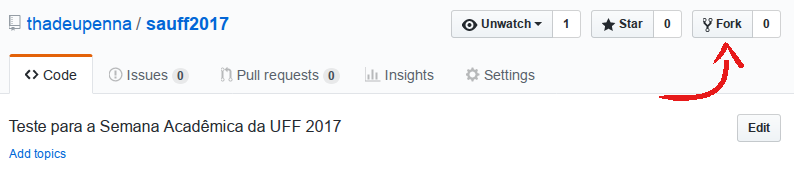
\includegraphics[width=\textwidth]{figures/fork}
\end{center}
\begin{itemize}
	\item Crie um fork do sauff2017
	\item Clone o seu repositório
	\item modifique o arquivo hello.c para imprimir seu nome
	\item Commite e envie para o GitHub.
	\item Faça um Pull Request e preencha os dados.
	\item Para continuar atualizando, adicione o repositório original com outro nome que não o origin (upstream, por exemplo).
\end{itemize}
\end{frame}


%
%
%
%%\begin{frame}{Git Rebase}
%%	Faz o mesmo que o merge (quando possível) mas tenta manter uma história linear. Bom para grandes projetos. \ttblue{git rebase -i} é interativo.
%%	\begin{center}
%%		\includegraphics[width=\textwidth]{rebase1}
%%	\end{center}
%%\end{frame}
%
%

\begin{frame}[fragile]{Comandos Úteis}
\begin{description}
		\item[\color{red}\ttblue{ git log --oneline --decorate --all --graph}] colore a saída do git log.
		\item[\ttblue{ git tag -d v1.0}] Apaga a tag.
		\item[\ttblue{ git push -{}-tags} ] Faz o upload das tags
		\item[\ttblue{ git remote show origin}] Informações sobre o repositório remoto.
		\item[\ttblue{ git fetch URL }] Pega os arquivos que ainda não foram atualizados mas não realiza um merge com o que você tem. Você deve fazer o merge manualmente.
        \item[\ttblue{git config --global credential.helper 'cache --timeout=3600'}] Não pergunta senha e usuário por uma hora .
\end{description}
\end{frame}

\end{document}
